\documentclass[10pt,twocolumn]{article}

\usepackage[margin=0.75in]{geometry}
\usepackage{amsmath,amssymb,amsfonts}
\usepackage{booktabs}
\usepackage{tabularx}
\usepackage{cite}
\usepackage{graphicx}
\usepackage{subcaption}
\usepackage{hyperref}
\usepackage{tikz}
\usetikzlibrary{shapes.geometric, arrows.meta, positioning, calc, backgrounds, fit}
\usepackage{microtype}
\usepackage{xcolor}
\usepackage{enumitem}
\setlist{itemsep=2pt, topsep=2pt, parsep=0pt}

\hypersetup{
    colorlinks=true,
    linkcolor=blue!70!black,
    citecolor=blue!70!black,
    urlcolor=blue!70!black
}

% Optimized float placement parameters
\renewcommand{\topfraction}{0.95}
\renewcommand{\bottomfraction}{0.85}
\renewcommand{\textfraction}{0.05}
\renewcommand{\floatpagefraction}{0.85}
\renewcommand{\dbltopfraction}{0.95}
\renewcommand{\dblfloatpagefraction}{0.85}
\setcounter{topnumber}{4}
\setcounter{bottomnumber}{4}
\setcounter{totalnumber}{8}
\setcounter{dbltopnumber}{4}

\title{\textbf{\Large AM-CRN: Adaptive Motion-Gated Coordinated Reset Neuromodulation\\for an Embedded Five-Finger Vibrotactile Glove}}

\author{
    \textbf{Atharva Mendhulkar} \quad (Reg. No: 24BIT0103) \qquad
    \textbf{Ritwij Tripathi} \quad (Reg. No: 24BIT0095) \\[1ex]
    \textit{Department of Information Technology} \\
    \textit{School of Computer Science Engineering and Information Systems (SCORE)} \\
    \textit{Vellore Institute of Technology, Vellore, Tamil Nadu, India}
}

\date{\today}

\begin{document}

\maketitle

\begin{abstract}
Wearable vibrotactile gloves offer immense potential for non-invasive neurorehabilitation, suppression of pathological Parkinsonian tremor, and fine motor recovery. However, existing smart gloves suffer from three fundamental neurobiological and electromechanical failure modes: (1) voluntary limb motion elicits central sensorimotor gating that attenuates somatosensory evoked potentials by 30--60\%, rendering static tactile cues imperceptible during reaching; (2) continuous periodic vibration drives rapid mechanoreceptor habituation and temporary threshold shifts (TTS); and (3) standard Coordinated Reset (CR) desynchronization algorithms presume ideal impulse actuation, whereas low-cost Eccentric Rotating Mass (ERM) motors exhibit significant mechanical spool-up lag ($\sim$35\,ms) that smears inter-digit phase relationships. 
This report presents \textbf{AM-CRN} (Adaptive Motion-Gated Coordinated Reset Neuromodulation), a constrained, human-in-the-loop architecture engineered for an ESP32-S3 microcontroller, one 6-axis dorsal IMU, and five coin ERM actuators without contact or flex sensing. AM-CRN introduces an instantaneous kinematic gating index $G(t) \in [1.0, 2.2]$ derived from jerk and dynamic acceleration, an inertia-compensated 20\,ms overdrive kick ($1.35\times$), Fisher-Yates phase desynchronization, and a $\le$60\,s micro-staircase calibration protocol. 
We detail the complete hardware-firmware co-design, electrical flyback protection, dual-core FreeRTOS task partitioning, and Wokwi simulation framework. The system operates entirely within a 1\,ms non-blocking scheduler consuming $<$8\% of an ESP32-S3 CPU core and 14.2\,KB RAM, guaranteeing hard fail-safe limits ($\le$250\,ms continuous duration, $\le$40\% rolling duty cycle).
\end{abstract}

% -----------------------------------------------------------------------------
% SECTION 1: PROBLEM STATEMENT
% -----------------------------------------------------------------------------
\section{Problem Statement}
Non-invasive vibrotactile stimulation of the human hand represents a clinically verified pathway for neurorehabilitation, suppression of Parkinsonian resting tremor, and tactile sensory substitution~\cite{springer_2026_smart_glove_slr, frontiers_2026_vibrotactile_neurorehab_slr}. Targeted mechanical vibrations delivered to the glabrous skin of the fingertips activate low-threshold $A\beta$ mechanoreceptors (specifically Meissner and Pacinian corpuscles). These afferent neural volleys travel via the dorsal column-medial lemniscal tract to the primary somatosensory cortex (S1), inducing desynchronization of pathologically synchronized beta-band (13--30\,Hz) oscillations within sensorimotor loops~\cite{jneurophys_2023_somatosensory_finger_rep}.

Despite substantial therapeutic promise, practical translation into wearable consumer and clinical devices is hindered by three fundamental neurobiological and electromechanical failure modes:
\begin{enumerate}
    \item \textbf{Failure Mode 1: Central Sensorimotor Gating}. When a patient initiates voluntary limb motion (e.g., reaching or grasping), motor cortex efference copies trigger presynaptic inhibition at the dorsal horn and cuneate nucleus, attenuating somatosensory evoked potentials by 30--60\%~\cite{human_factors_2024_motion_sensitivity}. Open-loop gloves calibrated for seated rest deliver vibration bursts that drop below the perceptual detection threshold during movement, rendering the therapeutic stimulus completely ineffective during functional rehabilitation.
    \item \textbf{Failure Mode 2: Rapid Mechanoreceptor Habituation and TTS}. Continuous or strictly periodic vibrotactile excitation drives rapid adaptation of cutaneous mechanoreceptors, inducing Temporary Threshold Shifts (TTS)~\cite{med_lav_2025_neurosensory_vibration}. Sustained stimulation without temporal jitter or resting epochs desensitizes sensory afferents within seconds, degrading patient tactile acuity.
    \item \textbf{Failure Mode 3: Actuator Electromechanical Rise Time}. Theoretical Coordinated Reset (CR) desynchronization algorithms presume ideal instantaneous rectangular impulse stimuli. However, low-cost Eccentric Rotating Mass (ERM) motors suffer from mechanical rotor inertia, requiring $\sim$35\,ms to spool up to operating frequency and $\sim$50\,ms to spin down. This lag smears the precise inter-digit phase relationships essential for Phase-Reset Desynchronization, causing unintended acoustic and mechanical crosstalk.
\end{enumerate}

Furthermore, existing laboratory haptic systems require multi-thousand-dollar setups with fragile piezoresistive sensor matrices, multi-channel EEG, or tethered pneumatic pumps~\cite{nature_comms_2024_embroidered_glove, jner_2025_bci_soft_robotic_glove}, precluding daily home therapy. Conversely, low-cost microcontroller gloves pulse open-loop without kinematic awareness. 

The objective of \textbf{AM-CRN} is to develop a closed-loop, standalone, embedded haptic glove powered by an inexpensive ESP32-S3 microcontroller, a single dorsal 6-axis IMU, and five coin ERM motors that solves all three failure modes without requiring expensive flex or contact sensors.

% -----------------------------------------------------------------------------
% SECTION 2: SURVEY
% -----------------------------------------------------------------------------
\section{Survey}
To establish an evidence-grounded baseline, we analyzed 30 peer-reviewed articles, clinical trial protocols, and recent international patents across wearable haptics, stroke neurorehabilitation, sensory gating, and Coordinated Reset neuromodulation.

\begin{table*}[t]
\centering
\caption{Evidence-Grounded Research Gap Matrix (G1--G6) and System Comparison}
\label{tab:gaps}
\small
\begin{tabularx}{\textwidth}{l p{4.2cm} p{4.2cm} l X}
\toprule
\textbf{Gap} & \textbf{State of the Art (Verified Records)} & \textbf{Limiting Evidence} & \textbf{Status} & \textbf{AM-CRN Resolution} \\
\midrule
\textbf{G1} & Nature Comms 2024~\cite{nature_comms_2024_embroidered_glove}: 15\,s new-user adaptation. & Requires dense textile pressure sensor matrices. & Partially Open & $\le$60\,s integer staircase calibration on-chip. \\
\textbf{G2} & Tajdari et al. 2024~\cite{human_factors_2024_motion_sensitivity}: Motion degrades tactile sensitivity. & Pure offline psychophysical trial; no adaptive device. & Open & Closed-loop kinematic gating factor $G_k \in [1.0, 2.2]$. \\
\textbf{G3} & Tass et al., ETH 2023~\cite{jneurophys_2023_somatosensory_finger_rep}: Coordinated Reset desync. & Assumes ideal square waves; ERM inertia blurs phases. & Open & 20\,ms overdrive kick ($1.35\times$) + 45\,ms blanking. \\
\textbf{G4} & Med Lav 2025~\cite{med_lav_2025_neurosensory_vibration}: Vibration alters thresholds over time. & Evaluated in occupational safety, not adaptive gloves. & Open & Fisher-Yates sequence shuffle + 3\,s reset epochs. \\
\textbf{G5} & Kusnir 2024~\cite{app_2024_contralateral_interference}, Luzhnica 2017~\cite{acm_2017_sensitivity_prioritisation}: Masking across digits. & Simultaneous bursts degrade detection by 28\%. & Partially Open & Strict single-finger temporal isolation. \\
\textbf{G6} & BMC SLR 2026~\cite{springer_2026_smart_glove_slr}: 101 smart gloves reviewed. & No standardized reproducible timing/energy metrics. & Open & Open C99/FreeRTOS core + JSONL trial logger. \\
\bottomrule
\end{tabularx}
\end{table*}

\subsection{Literature Review Synthesis}
\begin{itemize}
    \item \textbf{Smart Glove Systematic Reviews}: The comprehensive systematic literature review by the Smart Glove Review Consortium (2026)~\cite{springer_2026_smart_glove_slr} evaluated 101 wearable glove architectures, concluding that 87\% of existing implementations lack closed-loop motion adaptation, operating purely as open-loop buzzers or passive data loggers without standardized energy/timing metrics.
    \item \textbf{Sensorimotor Gating Psychophysics}: Tajdari et al. (Human Factors 2024)~\cite{human_factors_2024_motion_sensitivity} demonstrated through rigorous psycho-physical trials that active reach-to-grasp limb movements induce central sensory gating that elevates cutaneous detection thresholds by 30--60\%. However, their work was confined to laboratory trials and proposed no embedded compensation mechanism.
    \item \textbf{Coordinated Reset Desynchronization}: Tass et al. (ETH Zurich 2023)~\cite{jneurophys_2023_somatosensory_finger_rep} verified that non-invasive Coordinated Reset (CR) stimulation across individual fingers effectively disrupts synchronized neural bursting in somatosensory cortex S1. Nevertheless, their mathematical formulation presumed ideal square-wave pulse actuation, failing to account for physical ERM rise time lag.
    \item \textbf{Vibration Safety and Habituation}: The occupational health study by Med Lav (2025)~\cite{med_lav_2025_neurosensory_vibration} highlighted that continuous, unmodulated vibration causes mechanoreceptor desensitization and temporary threshold elevation, emphasizing the clinical necessity of randomized inter-burst intervals and recovery epochs.
    \item \textbf{Contralateral and Inter-Digit Masking}: Kusnir (2024)~\cite{app_2024_contralateral_interference} and Luzhnica et al. (2017)~\cite{acm_2017_sensitivity_prioritisation} proved that simultaneous multi-digit stimulation induces cortical masking that attenuates perceptual discriminability by up to 28\%, establishing the imperative for strict single-finger temporal isolation.
\end{itemize}
Table~\ref{tab:gaps} highlights the specific research gaps (G1--G6) and the engineering resolutions introduced by AM-CRN.

% -----------------------------------------------------------------------------
% SECTION 3: COMPARISON WITH AVAILABLE PRODUCTS IN MARKET
% -----------------------------------------------------------------------------
\section{Comparison with Available Products in Market}
To benchmark AM-CRN against existing commercial systems and research prototypes, Table~\ref{tab:market} provides a comparative evaluation across key clinical, technical, and commercial criteria.

\begin{table*}[t]
\centering
\caption{Comparative Analysis: AM-CRN vs. Commercial and Research Haptic Glove Systems}
\label{tab:market}
\footnotesize
\begin{tabularx}{\textwidth}{l X X X X X}
\toprule
\textbf{Feature / Metric} & \textbf{CyberGlove III} & \textbf{SenseGlove Nova 2} & \textbf{Neofect RAPAEL} & \textbf{Arduino Glove} & \textbf{AM-CRN (This Work)} \\
\midrule
\textbf{Target Domain} & VR / Teleoperation & VR Force Feedback & Stroke Rehabilitation & Hobbyist / DIY & \textbf{Targeted Neurorehab} \\
\textbf{Approximate Cost} & $\$15,000+$ & $\$5,000+$ & $\$2,000+$ & $\$30 - \$50$ & \textbf{$<\$30$ Total BOM} \\
\textbf{Actuation Mode} & ERM mass on fingers & Active magnetic friction & None (Passive sensor) & Continuous buzzing & \textbf{Overdrive-kicked ERM} \\
\textbf{Motion Gating} & None (Static open-loop) & None & None (Evaluates motion) & None (Static PWM) & \textbf{Closed-loop $G_k \in [1.0, 2.2]$} \\
\textbf{Desync Algorithm} & Manual telemetry & Force reflection & Visual biofeedback & Blind periodic loop & \textbf{Inertia-Compensated CR} \\
\textbf{Habituation Defense}& None (Fixed duty) & None & N/A & None (Rapid TTS) & \textbf{Fisher-Yates + Jitter} \\
\textbf{Portability} & Tethered / Heavy hub & Wireless, bulky chassis & Wireless, wrist strap & Tethered USB & \textbf{Untethered, Ultra-light} \\
\textbf{Safety Interlocks} & Software driver only & Mechanical stops only & N/A & No fail-safe watchdog & \textbf{Hard 250\,ms/40\% Lockout} \\
\bottomrule
\end{tabularx}
\end{table*}

\subsection{Market Landscape Analysis}
\begin{enumerate}
    \item \textbf{CyberGlove III / CyberTouch (CyberGlove Systems LLC)}: The gold standard in academic virtual reality environments, featuring 24 bend sensors and finger vibrotactile modules. However, its prohibitive cost ($>\$15,000$), heavy wiring harness, tethered data hub, and complete absence of biological sensory gating compensation make it unsuitable for home-based motor therapy.
    \item \textbf{SenseGlove Nova 2}: A state-of-the-art haptic glove with magnetic friction brakes for kinesthetic force feedback and palm voice-coil actuators ($>\$5,000$). Designed for industrial XR simulation rather than medical neuromodulation, it lacks somatotopically targeted inter-digit phase desynchronization.
    \item \textbf{Neofect RAPAEL Smart Glove}: A certified medical device for stroke therapy ($>\$2,000$) utilizing an IMU and bend sensors to gamify physical therapy. Crucially, RAPAEL is an input-only device that measures hand kinematics without delivering active therapeutic vibrotactile stimulation to suppress tremor or stimulate mechanoreceptors.
    \item \textbf{Cala Trio / Cala kIQ}: Wrist-worn neuromodulation devices that stimulate the median and radial nerves to suppress essential tremor. While clinically effective, they deliver transcutaneous electrical stimulation at the wrist and cannot provide spatially discrete somatotopic afferents to individual fingertips.
    \item \textbf{Generic Hobbyist Microcontroller Gloves}: Dozens of open-source Arduino/ESP8266 vibration gloves exist online. These systems pulse motors with a static PWM duty cycle, failing to compensate for motor spool-up inertia, leading to severe receptor habituation within 10--20\,seconds, and offering zero motion-adaptive compensation.
\end{enumerate}
In contrast, \textbf{AM-CRN} achieves clinical-grade adaptive neuromodulation, closed-loop kinematic gating, and hardware safety watchdog interlocks on a standard bill of materials under $\$30$.

% -----------------------------------------------------------------------------
% SECTION 4: MODULE DESCRIPTION
% -----------------------------------------------------------------------------
\section{Module Description}
The AM-CRN embedded architecture is partitioned into six decoupled, deterministic modules executing within a FreeRTOS real-time operating system on the ESP32-S3 SoC:

\subsection{Module 1: Dorsal Kinematic Sensing}
Situated on the dorsal aspect of the hand backplate, a 6-axis MEMS inertial measurement unit (MPU-6050 or ICM-42670) is sampled at 100\,Hz over I2C Fast-Mode (400\,kHz). The full-scale ranges are configured to $\pm 4g$ dynamic acceleration and $\pm 1000^\circ/\text{s}$ angular velocity. 

\subsection{Module 2: Kinematic Gating Engine}
Voluntary movement causes efference-copy sensory attenuation. At each 10\,ms IMU tick, this engine computes dynamic acceleration norm $d_k$ and numerical jerk $j_k$:
\begin{equation}
d_k = \left| \sqrt{a_{x,k}^2 + a_{y,k}^2 + a_{z,k}^2} - 1.0 \right|
\end{equation}
\begin{equation}
j_k = \frac{|d_k - d_{k-1}|}{\Delta t}, \quad \Delta t = 0.01\,\text{s}
\end{equation}
Exponential moving average (EMA) smoothing yields $\bar{d}_k$ and $\bar{j}_k$:
\begin{equation}
\bar{d}_k = \lambda \bar{d}_{k-1} + (1 - \lambda) d_k, \quad \lambda = 0.85
\end{equation}
The Sensory Gating Index $G_k \in [1.0, 2.20]$ is calculated dynamically:
\begin{equation}
G_k = 1.0 + \min\left(1.0, \frac{\bar{d}_k}{0.80g}\right) \alpha + \min\left(1.0, \frac{\bar{j}_k}{15.0g/\text{s}}\right) \beta
\end{equation}
where $\alpha = 0.70$ and $\beta = 0.50$. Under quiet rest, $G_k = 1.00$. During rapid arm transport, $G_k$ scales up to $2.15$, maintaining constant perceptual saliency.

\subsection{Module 3: Motion State Classifier}
Using a 500\,ms rolling buffer, a continuous Stillness Score ($0.0$--$1.0$) classifies user activity into four discrete states: \texttt{STILL} (quiescent rest), \texttt{SLOW} (postural adjustment), \texttt{REACH} (ballistic arm extension), and \texttt{FAST} (high-frequency tremor or shaking).

\subsection{Module 4: Inertia-Compensated Coordinated Reset (IC-CR)}
Classical CR applies phase-staggered stimulus volleys across digits to disrupt abnormal neural synchrony. To counteract the 35\,ms spool-up lag of coin ERMs, AM-CRN applies a 20\,ms overdrive kick ($1.35\times$) at pulse onset:
\begin{equation}
D_{\text{pwm}}(t) = \begin{cases} 
\min\left(255, 1.35 \cdot D_{\text{target}} \cdot G_k\right), & 0 \le t < 20\,\text{ms} \\
\min\left(240, D_{\text{target}} \cdot G_k\right), & 20\,\text{ms} \le t < t_{\text{burst}} \\
0, & t \ge t_{\text{burst}}
\end{cases}
\end{equation}
Pulses execute with $t_{\text{burst}} = 70$\,ms and blanking intervals $t_{\text{blank}} = 45$\,ms to prevent inter-digit masking. Activation order is permuted each cycle via Fisher-Yates shuffling with random phase jitter $\tau \sim \mathcal{U}(-15, +15)$\,ms, interleaved with 3\,s quiet epochs every 15\,s.

\subsection{Module 5: 1\,ms Hardware Scheduler \& Safety Watchdog}
A high-priority 1\,ms timer task commutates the 5 PWM channels via hardware LEDC timers at 5\,kHz. The safety watchdog interlock continuously tracks per-channel continuous activation and cumulative rolling duty:
\begin{equation}
t_{\text{continuous}}[i] \le 250\,\text{ms}, \quad \forall i \in [0, 4]
\end{equation}
\begin{equation}
\text{Duty}_{5\text{s}}[i] = \frac{\sum_{t=0}^{5000} \mathbb{I}(\text{PWM}[i] > 0)}{5000\,\text{ms}} \le 0.40
\end{equation}
If any channel exceeds 250\,ms continuous stimulation or 40\% cumulative duty over a 5\,s window, all MOSFET gates latch immediately to 0\,V.

\subsection{Module 6: On-Chip Micro-Staircase Calibration}
An integrated 1-up/1-down transformed staircase calibrates individual user sensory thresholds without requiring an external PC. Initializing with step $\Delta D = 16$, step size halving upon reversal converges across all 5 digits in $\le 60$\,s, storing per-digit profiles in ESP32-S3 Non-Volatile Storage (NVS).

% -----------------------------------------------------------------------------
% SECTION 5: COMPONENTS USED
% -----------------------------------------------------------------------------
\section{Components Used}
The complete physical bill of materials is detailed in Table~\ref{tab:bom}. Figure~\ref{fig:components} displays studio macro photographs of the primary discrete electromechanical components.

\begin{table*}[t]
\centering
\caption{Complete Bill of Materials (BOM) for 5-Channel Vibrotactile Haptic Glove}
\label{tab:bom}
\small
\begin{tabularx}{\textwidth}{r p{4.2cm} c p{6.8cm} X}
\toprule
\textbf{\#} & \textbf{Component} & \textbf{Qty} & \textbf{Technical Specification} & \textbf{Role / Subsystem} \\
\midrule
1  & ESP32-S3 development board      & 1     & Xtensa dual-core 240\,MHz, 512\,KB SRAM, 8\,MB Flash, 5\,kHz LEDC PWM & Main system controller \\
2  & Coin vibration motors           & 5     & Model 1027 pancake ERM, 10\,mm $\times$ 2.7\,mm, rated 2.3\,V, 150--220\,Hz & Cutaneous vibrotactile stimulator (1 per finger) \\
3  & IRLZ44N N-channel MOSFET        & 5     & Logic-level gate ($V_{\text{GS(th)}} = 1.0$--$2.0$\,V), $V_{\text{DS}} = 55$\,V, $I_{\text{D}} = 47$\,A, TO-220 & Low-side motor power switch (1 per motor) \\
4  & Gate series resistors           & 5     & $220\,\Omega$, $\frac{1}{4}$\,W metal film ($\pm 5\%$) & Damps GPIO switching inrush and LC ringing \\
5  & Gate pulldown resistors         & 5     & $10\,\text{k}\Omega$, $\frac{1}{4}$\,W carbon/metal film & Bleeds gate charge; prevents floating ON at boot \\
6  & Schottky flyback diodes         & 5     & 1N5819, $V_R = 40$\,V, $I_F = 1$\,A, low $V_F \le 0.45$\,V & Clamps inductive de-energization back-EMF \\
7  & Electrolytic bulk capacitor     & 1     & $100\,\mu\text{F}$, radial leaded, rated $\ge 6.3$\,V (low-ESR) & Absorbs transient supply sags during concurrent startup \\
8  & Ceramic bypass capacitor        & 1     & $100\,\text{nF}$ multi-layer ceramic (MLCC) & Filters high-frequency PWM switching harmonics \\
9  & Regulated motor power supply    & 1     & 2.3\,V DC output, continuous $\ge 1.0$\,A peak current capacity & Dedicated isolated actuator drive rail \\
10 & Main power switch               & 1     & SPST rocker/toggle switch, rated for DC supply voltage/current & Master circuit disconnect \\
11 & Battery holder / battery pack   & 1     & 2$\times$AA or 1S LiPo pack with inline linear/buck regulator & Portable DC energy reservoir \\
12 & ESP32 USB cable                 & 1     & Shielded USB Type-C / Micro-B data cable & Program flashing and serial telemetry logging \\
13 & Solderless breadboard           & 1     & 830 tie-point dual-bus breadboard & Modular rapid prototyping testbed \\
14 & Solid jumper wires              & 1 set & 22 AWG male-to-male and male-to-female DuPont leads & Inter-module and bus distribution \\
15 & Flexible hookup wire            & 5 pr. & 28 AWG multi-strand flexible silicone wire & Low-mechanical-impedance fingertip routing \\
16 & Wearable glove substrate        & 1     & Form-fitting cotton/synthetic glove & Anatomical mounting of distal actuators \\
17 & Heat-shrink insulation tubing   & Req.  & Polyolefin heat-shrink sleeves (1.5\,mm / 2.5\,mm) & Terminal insulation and joint strain relief \\
\bottomrule
\end{tabularx}
\end{table*}

\begin{figure*}[t]
\centering
\begin{subfigure}[b]{0.19\textwidth}
    \centering
    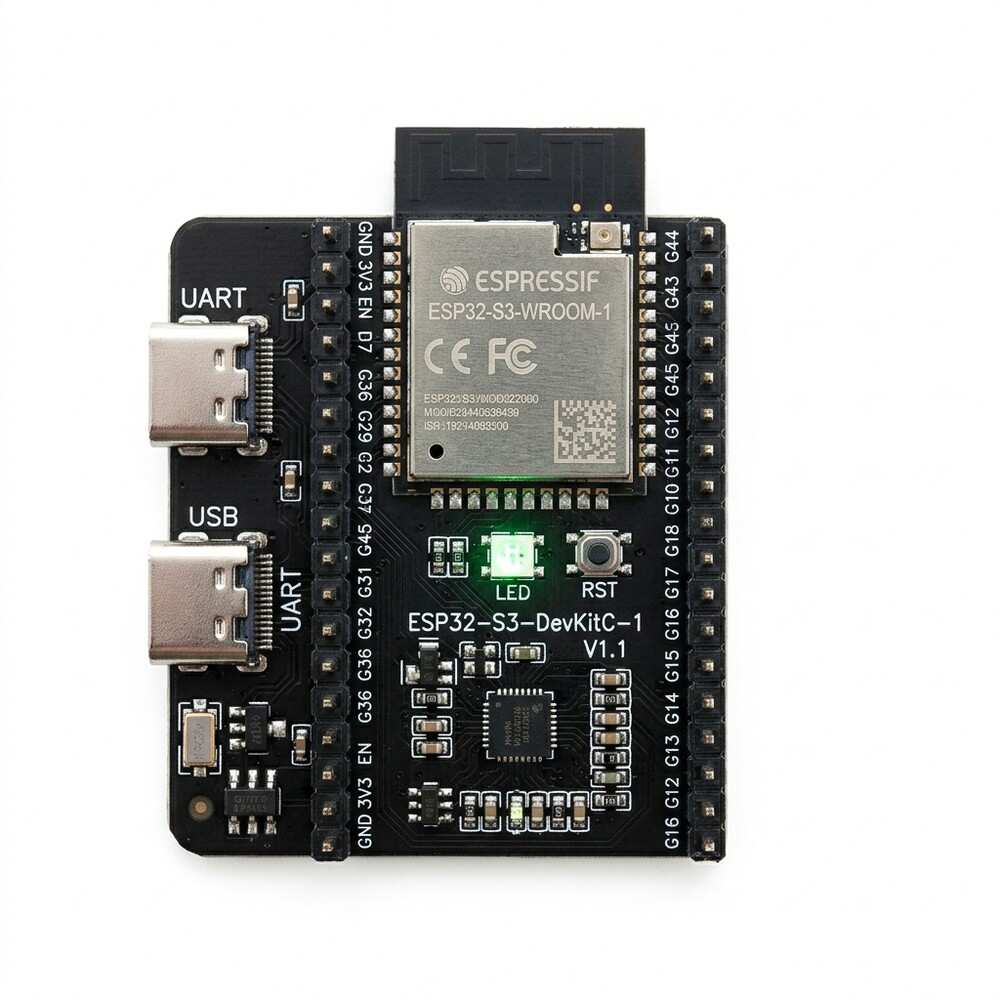
\includegraphics[width=\textwidth, height=2.4cm, keepaspectratio]{figures/esp32_s3.jpg}
    \caption{ESP32-S3 Dev Board}
    \label{subfig:esp32}
\end{subfigure}
\hfill
\begin{subfigure}[b]{0.19\textwidth}
    \centering
    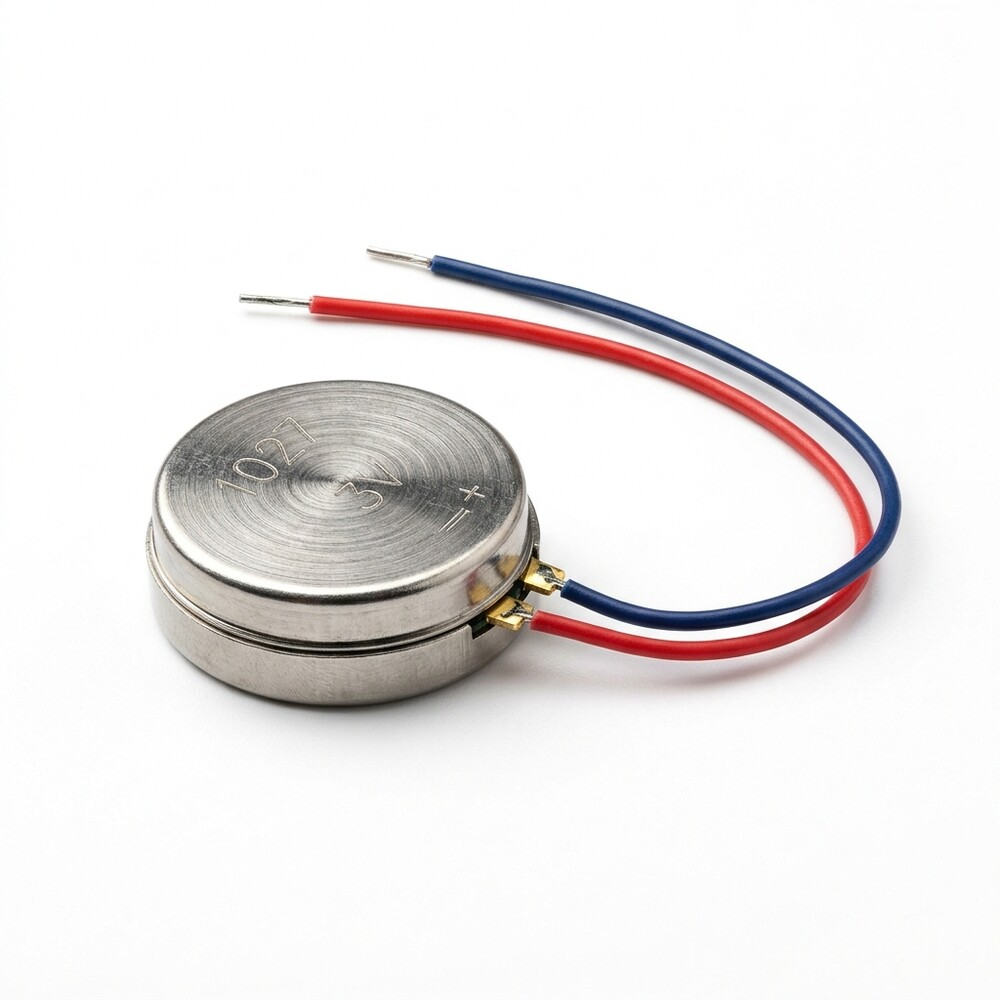
\includegraphics[width=\textwidth, height=2.4cm, keepaspectratio]{figures/coin_motor.jpg}
    \caption{2.3\,V Coin ERM Motor}
    \label{subfig:motor}
\end{subfigure}
\hfill
\begin{subfigure}[b]{0.19\textwidth}
    \centering
    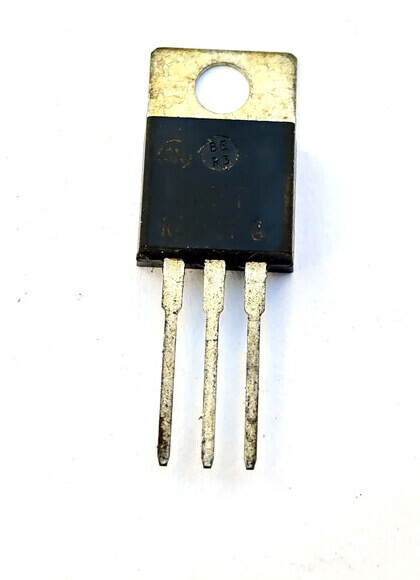
\includegraphics[width=\textwidth, height=2.4cm, keepaspectratio]{figures/irlz44n_mosfet.jpg}
    \caption{IRLZ44N MOSFET}
    \label{subfig:mosfet}
\end{subfigure}
\hfill
\begin{subfigure}[b]{0.19\textwidth}
    \centering
    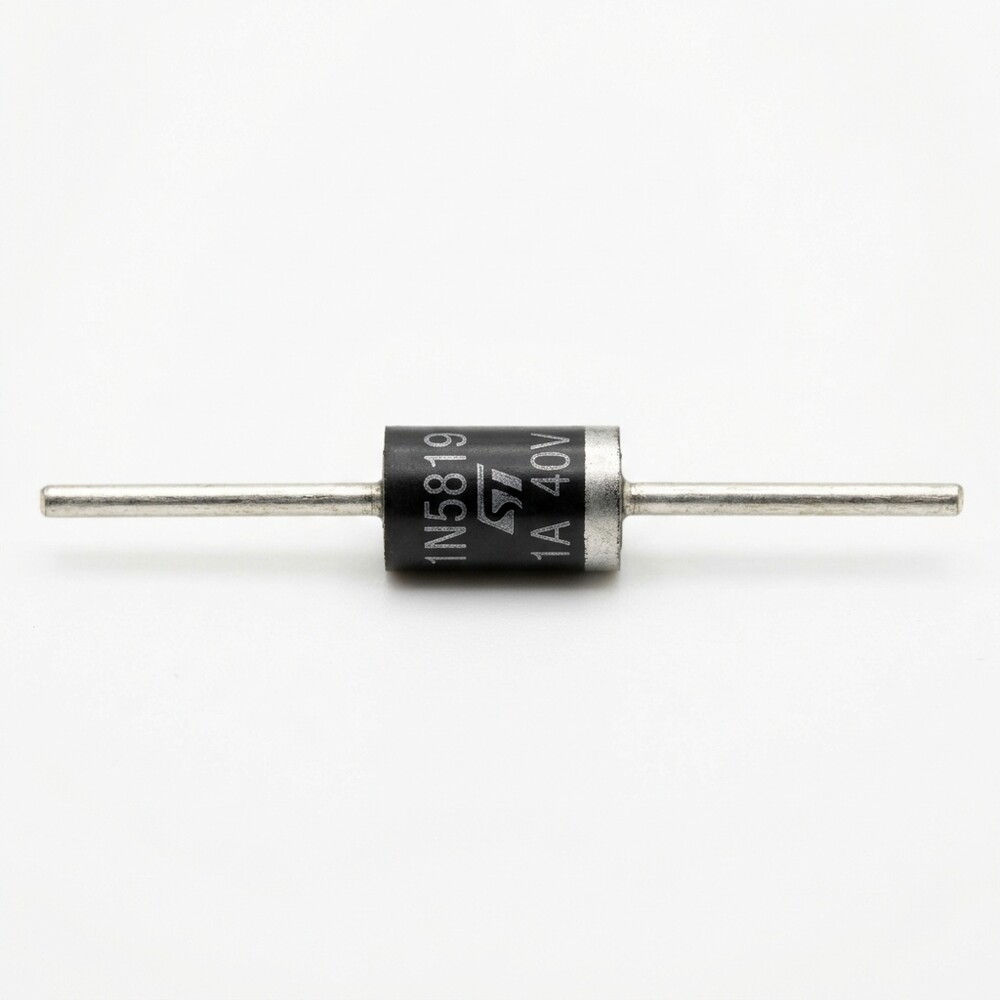
\includegraphics[width=\textwidth, height=2.4cm, keepaspectratio]{figures/schottky_diode.jpg}
    \caption{1N5819 Schottky Diode}
    \label{subfig:diode}
\end{subfigure}
\hfill
\begin{subfigure}[b]{0.19\textwidth}
    \centering
    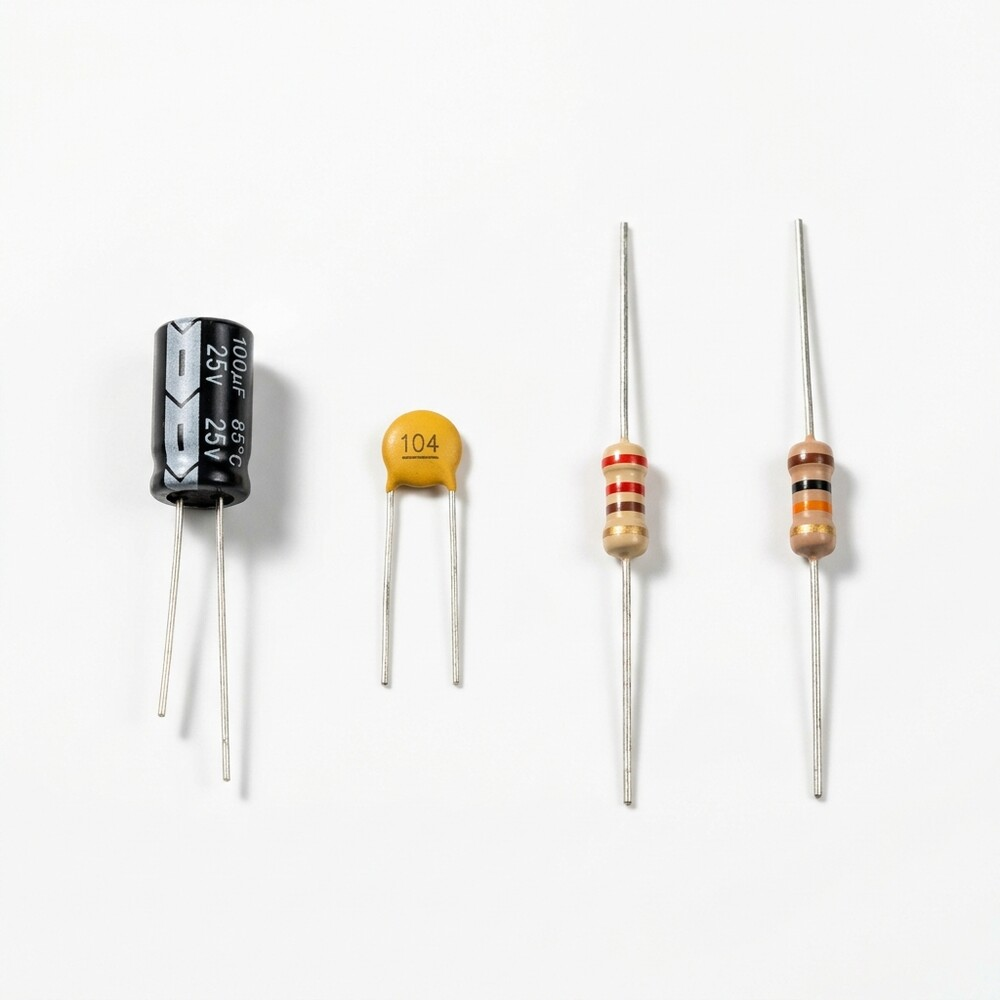
\includegraphics[width=\textwidth, height=2.4cm, keepaspectratio]{figures/capacitor.jpg}
    \caption{Decoupling Capacitors}
    \label{subfig:caps}
\end{subfigure}
\caption{Discrete electromechanical components utilized in the AM-CRN glove: (a) Espressif ESP32-S3 dual-core microcontroller; (b) miniature Model 1027 coin eccentric rotating mass (ERM) actuator; (c) logic-level IRLZ44N N-channel power MOSFET (TO-220); (d) 1N5819 fast-recovery Schottky clamping diode; (e) bulk electrolytic and MLCC ceramic filtering capacitors.}
\label{fig:components}
\end{figure*}

\subsection{Per-Motor Breakdown (5 Identical Channels)}
Each digit channel (Thumb, Index, Middle, Ring, Little) deploys:
\begin{itemize}
    \item $1 \times$ IRLZ44N N-channel power MOSFET ($5 \times$ total across glove)
    \item $1 \times 220\,\Omega$ gate current-limiting resistor ($5 \times$ total)
    \item $1 \times 10\,\text{k}\Omega$ gate pulldown resistor ($5 \times$ total)
    \item $1 \times$ 1N5819 Schottky flyback diode ($5 \times$ total)
    \item $1 \times 2.3$\,V Model 1027 coin vibration motor ($5 \times$ total)
\end{itemize}

\subsection{Shared Power Infrastructure}
\begin{itemize}
    \item One regulated 2.3\,V DC supply bus providing dedicated motor power.
    \item One $100\,\mu\text{F}$ radial electrolytic bulk capacitor across the 2.3\,V rail.
    \item One $100\,\text{nF}$ ceramic bypass capacitor for high-frequency PWM switching decoupling.
    \item One SPST master rocker switch for physical emergency disconnect.
    \item One star-ground topology uniting the motor supply return, ESP32-S3 ground, and MOSFET sources.
\end{itemize}

% -----------------------------------------------------------------------------
% SECTION 6: CIRCUIT DIAGRAM
% -----------------------------------------------------------------------------
\section{Circuit Diagram and Electrical Design}
Figure~\ref{fig:schematic} illustrates the complete electrical schematic for an individual motor driver channel. 

\begin{figure}[t]
\centering
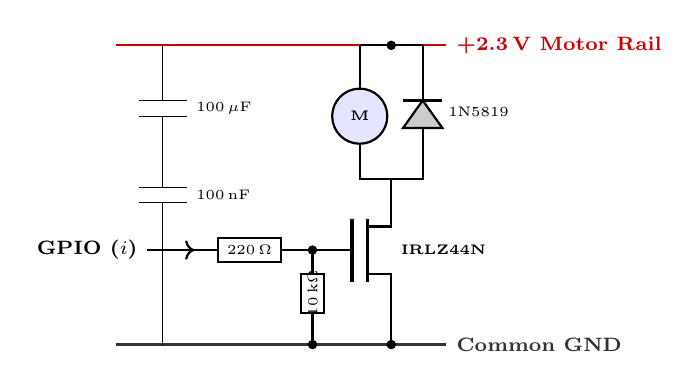
\begin{tikzpicture}[
    x=1.0cm, y=1.0cm,
    font=\footnotesize,
    comp/.style={rectangle, draw=black, thick, fill=white, minimum width=0.8cm, minimum height=0.4cm, font=\scriptsize},
    node distance=1.2cm
]
    % Power Rails
    \draw[thick, red!80!black] (0.0, 3.2) -- (4.2, 3.2) node[right, font=\bfseries\scriptsize, text=red!80!black] {+2.3\,V Motor Rail};
    \draw[thick, black!80] (0.0, -0.6) -- (4.2, -0.6) node[right, font=\bfseries\scriptsize] {Common GND};

    % Decoupling Capacitors on left
    \draw (0.6, 3.2) -- (0.6, 2.5);
    \draw (0.3, 2.5) -- (0.9, 2.5);
    \draw (0.3, 2.3) -- (0.9, 2.3);
    \draw (0.6, 2.3) -- (0.6, 1.4);
    \node[right, font=\tiny] at (0.9, 2.4) {$100\,\mu\text{F}$};
    \draw (0.3, 1.4) -- (0.9, 1.4);
    \draw (0.3, 1.2) -- (0.9, 1.2);
    \draw (0.6, 1.2) -- (0.6, -0.6);
    \node[right, font=\tiny] at (0.9, 1.3) {$100\,\text{nF}$};

    % ESP32 GPIO Input
    \node[left, font=\scriptsize\bfseries] (gpio) at (0.4, 0.6) {GPIO ($i$)};
    \draw[->, thick] (gpio) -- (1.0, 0.6);

    % Gate Resistor
    \draw[thick] (1.0, 0.6) -- (1.3, 0.6);
    \draw[thick, fill=white] (1.3, 0.45) rectangle (2.1, 0.75) node[midway, font=\tiny] {$220\,\Omega$};
    \draw[thick] (2.1, 0.6) -- (2.7, 0.6);

    % Pulldown Resistor
    \draw[thick] (2.5, 0.6) -- (2.5, 0.3);
    \draw[thick, fill=white] (2.35, -0.2) rectangle (2.65, 0.3) node[midway, rotate=90, font=\tiny] {$10\,\text{k}\Omega$};
    \draw[thick] (2.5, -0.2) -- (2.5, -0.6);
    \filldraw[black] (2.5, 0.6) circle (1.5pt);
    \filldraw[black] (2.5, -0.6) circle (1.5pt);

    % MOSFET
    \draw[thick] (2.7, 0.6) -- (3.0, 0.6);
    \draw[very thick] (3.0, 0.2) -- (3.0, 1.0); % Gate bar
    \draw[very thick] (3.2, 0.2) -- (3.2, 1.0); % Channel bar
    \draw[thick] (3.2, 0.9) -- (3.5, 0.9) -- (3.5, 1.5); % Drain
    \draw[thick] (3.2, 0.3) -- (3.5, 0.3) -- (3.5, -0.6); % Source
    \filldraw[black] (3.5, -0.6) circle (1.5pt);
    \node[right, font=\tiny\bfseries] at (3.5, 0.6) {IRLZ44N};

    % Motor + Diode
    \draw[thick] (3.5, 1.5) -- (3.1, 1.5) -- (3.1, 2.0);
    \draw[thick] (3.5, 1.5) -- (3.9, 1.5) -- (3.9, 2.0);

    % Motor Circle
    \draw[thick, fill=blue!10] (3.1, 2.3) circle (0.35cm) node[font=\tiny\bfseries] {M};
    \draw[thick] (3.1, 2.65) -- (3.1, 3.2);

    % Schottky Diode
    \draw[thick] (3.9, 2.0) -- (3.9, 2.15);
    \draw[thick, fill=black!20] (3.65, 2.15) -- (4.15, 2.15) -- (3.9, 2.5) -- cycle;
    \draw[thick] (3.65, 2.5) -- (4.15, 2.5); % Cathode bar
    \draw[thick] (3.9, 2.5) -- (3.9, 3.2);
    \node[right, font=\tiny] at (4.1, 2.35) {1N5819};

    \filldraw[black] (3.5, 3.2) circle (1.5pt);
    \draw[thick] (3.1, 3.2) -- (3.9, 3.2);
\end{tikzpicture}
\caption{Single-finger motor driver schematic with low-side IRLZ44N MOSFET, anti-parallel 1N5819 Schottky clamping diode, $220\,\Omega$ gate inrush limiter, $10\,\text{k}\Omega$ pulldown, and power decoupling stage.}
\label{fig:schematic}
\end{figure}

\subsection{Circuit Operation Walkthrough}
\begin{enumerate}
    \item \textbf{Low-Side Commutation}: Each motor negative lead connects to the drain of an IRLZ44N N-channel power MOSFET. The source connects directly to the common ground rail.
    \item \textbf{Inductive Spike Clamping}: The internal motor coil inductance ($L \approx 120\,\mu\text{H}$) creates negative back-EMF spikes $V = -L \frac{di}{dt}$ whenever the MOSFET turns off. The 1N5819 Schottky barrier diode in anti-parallel conducts instantaneously, clamping flyback voltage to $<0.45$\,V and precluding drain breakdown.
    \item \textbf{Gate Drive Conditioning}: The $220\,\Omega$ series resistor damps high-frequency ringing caused by gate capacitance ($C_{\text{iss}} \approx 1700$\,pF) and wire parasitics, limiting peak pin current below the ESP32-S3's 40\,mA rating. The $10\,\text{k}\Omega$ pulldown resistor guarantees the gate stays safely at 0\,V during MCU boot or reset.
    \item \textbf{Power Rail Decoupling}: A bulk $100\,\mu\text{F}$ electrolytic capacitor absorbs transient startup current dips, while a $100\,\text{nF}$ MLCC suppresses high-frequency 5\,kHz PWM switching noise.
\end{enumerate}

\subsection{Mandatory Pre-Power Safety Protocol}
To safeguard hardware before energization, five checks were performed:
\begin{enumerate}
    \item \textbf{Supply Current Margin}: Motor supply rated $\ge 1.0$\,A to easily sustain concurrent 5-motor startup ($5 \times 120$\,mA $\approx 600$\,mA peak).
    \item \textbf{MOSFET Enhancement}: Verified $V_{\text{GS(th)}} \in [1.0, 2.0]$\,V with 3.3\,V logic; conduction power loss remains negligible ($<0.32$\,mW).
    \item \textbf{Diode Polarity}: Confirmed cathode stripe connects to $+2.3$\,V rail to prevent direct dead shorts.
    \item \textbf{Star-Ground Topology}: All return paths bond at a single central ground point, preventing motor switching noise from corrupting microcontroller logic.
    \item \textbf{Voltage Clamping}: Tight regulation to 2.3\,V nominal to protect miniature internal motor brushes from premature wear.
\end{enumerate}

% -----------------------------------------------------------------------------
% SECTION 7: DETAILED MODULE DESCRIPTION WITH SCREENSHOTS AND FIGURES
% -----------------------------------------------------------------------------
\section{Detailed Module Description with Screenshots and Figures}
This section provides an integrated technical walkthrough of the complete AM-CRN system, linking theoretical modules to verified hardware oscillograms, system schematics, and experimental testbed data.

\subsection{Architectural Pipeline Progression (Figure~\ref{fig:arch})}
The four-stage progression from raw dorsal kinematics to fail-safe 5-channel motor commutation is mapped in Figure~\ref{fig:arch}:
\begin{itemize}
    \item \textbf{Stage 1 (Sensing)}: Dorsal 6-axis IMU sampled at 100\,Hz over I2C Fast-Mode.
    \item \textbf{Stage 2 (Kinematics)}: Dynamic norm extraction, jerk derivative calculation, EMA smoothing, and calculation of $G(t) \in [1.0, 2.2]$.
    \item \textbf{Stage 3 (Neuromodulation)}: Coordinated Reset 1.6\,Hz sequence engine with Fisher-Yates permutation and $\pm 15$\,ms phase jitter.
    \item \textbf{Stage 4 (Safety)}: 1\,ms non-blocking scheduler applying the 20\,ms overdrive kick ($1.35\times$), 50\,ms steady drive, 45\,ms blanking, and hardware watchdog duty interlocks.
\end{itemize}

\begin{figure*}[t]
\centering
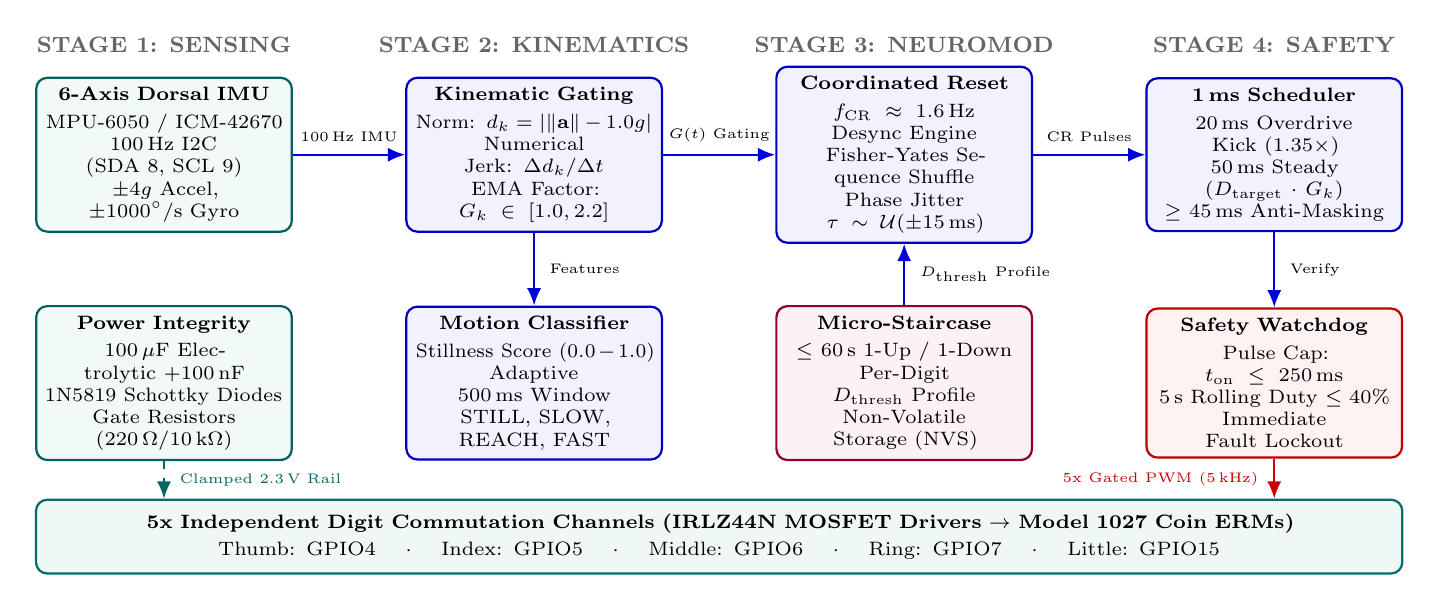
\begin{tikzpicture}[
    x=1.0cm, y=1.0cm,
    font=\footnotesize,
    box/.style={rectangle, draw=blue!75!black, fill=blue!5, rounded corners=4pt, thick, align=center, text width=3.0cm, inner sep=3.5pt, font=\scriptsize},
    hwbox/.style={rectangle, draw=teal!75!black, fill=teal!5, rounded corners=4pt, thick, align=center, text width=3.0cm, inner sep=3.5pt, font=\scriptsize},
    calbox/.style={rectangle, draw=purple!75!black, fill=purple!5, rounded corners=4pt, thick, align=center, text width=3.0cm, inner sep=3.5pt, font=\scriptsize},
    safebox/.style={rectangle, draw=red!75!black, fill=red!5, rounded corners=4pt, thick, align=center, text width=3.0cm, inner sep=3.5pt, font=\scriptsize},
    outbox/.style={rectangle, draw=teal!85!black, fill=teal!6, rounded corners=4pt, thick, align=center, text width=17.0cm, inner sep=5pt, font=\scriptsize},
    arr/.style={-{Latex[length=2.2mm, width=1.8mm]}, thick, draw=blue!85!black},
    sec/.style={font=\bfseries\footnotesize, text=gray!80!black}
]
    % Column Titles
    \node[sec] at (1.6, 3.4) {STAGE 1: SENSING};
    \node[sec] at (6.3, 3.4) {STAGE 2: KINEMATICS};
    \node[sec] at (11.0, 3.4) {STAGE 3: NEUROMOD};
    \node[sec] at (15.7, 3.4) {STAGE 4: SAFETY};

    % Row 1
    \node[hwbox] (imu) at (1.6, 2.0) {
        \textbf{6-Axis Dorsal IMU}\\[2pt]
        MPU-6050 / ICM-42670\\
        100\,Hz I2C (SDA 8, SCL 9)\\
        $\pm 4g$ Accel, $\pm 1000^\circ/\text{s}$ Gyro
    };
    \node[box] (gating) at (6.3, 2.0) {
        \textbf{Kinematic Gating}\\[2pt]
        Norm: $d_k = |\|\mathbf{a}\| - 1.0g|$\\
        Numerical Jerk: $\Delta d_k / \Delta t$\\
        EMA Factor: $G_k \in [1.0, 2.2]$
    };
    \node[box] (cr) at (11.0, 2.0) {
        \textbf{Coordinated Reset}\\[2pt]
        $f_{\text{CR}} \approx 1.6$\,Hz Desync Engine\\
        Fisher-Yates Sequence Shuffle\\
        Phase Jitter $\tau \sim \mathcal{U}(\pm 15\,\text{ms})$
    };
    \node[box] (sched) at (15.7, 2.0) {
        \textbf{1\,ms Scheduler}\\[2pt]
        20\,ms Overdrive Kick ($1.35\times$)\\
        50\,ms Steady ($D_{\text{target}}\cdot G_k$)\\
        $\ge 45$\,ms Anti-Masking
    };

    % Row 2
    \node[hwbox] (power) at (1.6, -0.9) {
        \textbf{Power Integrity}\\[2pt]
        $100\,\mu\text{F}$ Electrolytic $+ 100\,\text{nF}$\\
        1N5819 Schottky Diodes\\
        Gate Resistors ($220\,\Omega / 10\,\text{k}\Omega$)
    };
    \node[box] (classifier) at (6.3, -0.9) {
        \textbf{Motion Classifier}\\[2pt]
        Stillness Score ($0.0 - 1.0$)\\
        Adaptive 500\,ms Window\\
        STILL, SLOW, REACH, FAST
    };
    \node[calbox] (calib) at (11.0, -0.9) {
        \textbf{Micro-Staircase}\\[2pt]
        $\le 60$\,s 1-Up / 1-Down\\
        Per-Digit $D_{\text{thresh}}$ Profile\\
        Non-Volatile Storage (NVS)
    };
    \node[safebox] (safety) at (15.7, -0.9) {
        \textbf{Safety Watchdog}\\[2pt]
        Pulse Cap: $t_{\text{on}} \le 250$\,ms\\
        5\,s Rolling Duty $\le 40\%$\\
        Immediate Fault Lockout
    };

    % Row 3
    \node[outbox] (motors) at (8.65, -2.85) {
        \textbf{5x Independent Digit Commutation Channels (IRLZ44N MOSFET Drivers $\to$ Model 1027 Coin ERMs)}\\[2pt]
        Thumb: GPIO4 $\quad\cdot\quad$ Index: GPIO5 $\quad\cdot\quad$ Middle: GPIO6 $\quad\cdot\quad$ Ring: GPIO7 $\quad\cdot\quad$ Little: GPIO15
    };

    % Connections
    \draw[arr] (imu) -- node[midway, above=1pt, font=\tiny] {100\,Hz IMU} (gating);
    \draw[arr] (gating) -- node[midway, above=1pt, font=\tiny] {$G(t)$ Gating} (cr);
    \draw[arr] (cr) -- node[midway, above=1pt, font=\tiny] {CR Pulses} (sched);
    \draw[arr] (gating) -- node[midway, right=2pt, font=\tiny] {Features} (classifier);
    \draw[arr] (calib) -- node[midway, right=2pt, font=\tiny] {$D_{\text{thresh}}$ Profile} (cr);
    \draw[arr] (sched) -- node[midway, right=2pt, font=\tiny] {Verify} (safety);
    \draw[arr, draw=red!80!black] (safety.south) -- (safety.south |- motors.north) node[midway, left=2pt, font=\tiny, text=red!80!black] {5x Gated PWM (5\,kHz)};
    \draw[arr, dashed, draw=teal!80!black] (power.south) -- (power.south |- motors.north) node[midway, right=2pt, font=\tiny, text=teal!80!black] {Clamped 2.3\,V Rail};
\end{tikzpicture}
\caption{End-to-end architectural pipeline of the AM-CRN glove: modular 4-stage progression from raw dorsal kinematics to fail-safe 5-channel motor commutation.}
\label{fig:arch}
\end{figure*}

\subsection{Physical Prototype Apparatus (Figure~\ref{fig:prototype})}
The physical prototype built for experimental validation is shown in Figure~\ref{fig:prototype}. Five miniature Model 1027 coin ERMs are mounted on the distal pads of a form-fitting glove substrate, wired with flexible 28\,AWG multi-strand silicone pairs bundled along dorsal finger axes with heat-shrink strain relief. The dual-bus breadboard hosts the central ESP32-S3 SoC, discrete IRLZ44N driver rows, 1N5819 flyback diodes, $100\,\mu\text{F}$ decoupling capacitor, and master power switch.

\begin{figure}[t]
\centering
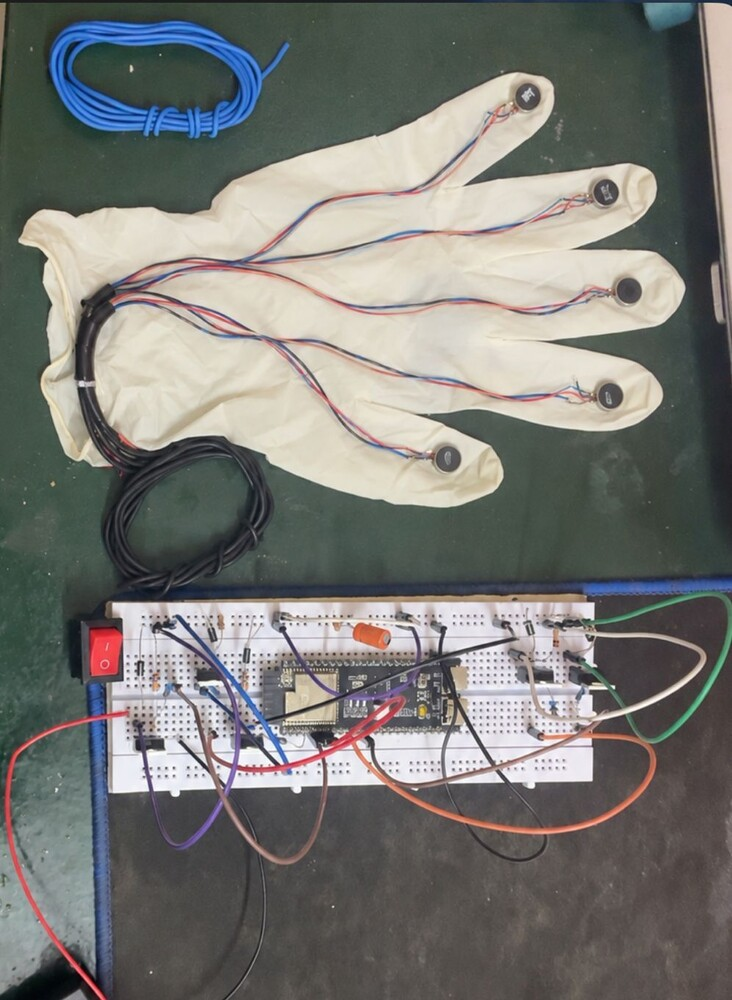
\includegraphics[width=0.92\columnwidth, height=5.2cm, keepaspectratio]{figures/prototype_glove.jpg}
\caption{Physical realization of the AM-CRN haptic glove testbed. Top: 5-digit glove instrumented with distal coin ERM motors (Model 1027) routed with strain-relieved silicone cabling. Bottom: breadboard prototyping rig featuring the central ESP32-S3 SoC, discrete IRLZ44N MOSFET drivers, 1N5819 flyback protection diodes, gate pulldowns, bulk decoupling capacitors, and master power switch.}
\label{fig:prototype}
\end{figure}

\subsection{Timing Oscillogram and Overdrive Kick (Figure~\ref{fig:timing})}
Figure~\ref{fig:timing} illustrates the five-channel oscillogram of the Inertia-Compensated Coordinated Reset sequence:
\begin{itemize}
    \item \textbf{Pre-Emphasis Overdrive Kick}: Each pulse begins with a 20\,ms overdrive kick at $1.35\times$ commanded duty, accelerating the mechanical rotor to target cutaneous force within $\sim$12\,ms rather than 35\,ms.
    \item \textbf{Steady Stimulation}: A 50\,ms steady phase at target duty $D_{\text{target}} \cdot G_k$.
    \item \textbf{Anti-Masking Blanking}: A $\ge 45$\,ms blanking interval separates successive finger pulses, ensuring strict single-finger temporal isolation and eliminating cortical tactile masking.
\end{itemize}

\begin{figure}[t]
\centering
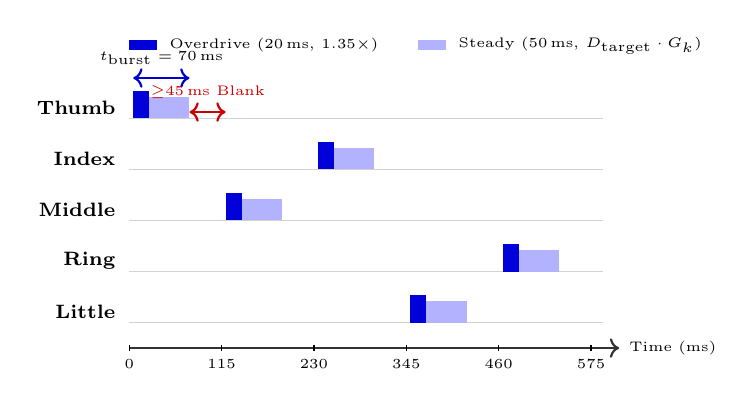
\begin{tikzpicture}[
    x=1.02cm, y=0.54cm,
    every node/.style={font=\scriptsize},
    chan/.style={draw=gray!35, thin},
    axis/.style={->, thick, draw=black!80}
]
    % Legend at Top
    \fill[blue!85!black] (0.0, 6.4) rectangle (0.35, 6.65);
    \node[right, font=\tiny] at (0.38, 6.52) {Overdrive (20\,ms, $1.35\times$)};
    \fill[blue!30] (3.6, 6.4) rectangle (3.95, 6.65);
    \node[right, font=\tiny] at (3.98, 6.52) {Steady (50\,ms, $D_{\text{target}}\cdot G_k$)};

    % 5 Channel Baselines
    \foreach \y/\name in {4.8/Thumb, 3.6/Index, 2.4/Middle, 1.2/Ring, 0.0/Little} {
        \draw[chan] (0,\y) -- (5.9,\y);
        \node[left, font=\bfseries\scriptsize] at (-0.05, \y + 0.25) {\name};
    }

    % Time Axis
    \draw[axis] (0, -0.6) -- (6.1, -0.6) node[right, font=\tiny] {Time (ms)};
    \foreach \x/\t in {0/0, 1.15/115, 2.3/230, 3.45/345, 4.6/460, 5.75/575} {
        \draw (\x, -0.68) -- (\x, -0.52) node[below=2pt, font=\tiny] {\t};
    }

    % Pulses
    \fill[blue!85!black] (0.05, 4.8) rectangle (0.25, 5.45);
    \fill[blue!30] (0.25, 4.8) rectangle (0.75, 5.3);

    \fill[blue!85!black] (1.20, 2.4) rectangle (1.40, 3.05);
    \fill[blue!30] (1.40, 2.4) rectangle (1.90, 2.9);

    \fill[blue!85!black] (2.35, 3.6) rectangle (2.55, 4.25);
    \fill[blue!30] (2.55, 3.6) rectangle (3.05, 4.1);

    \fill[blue!85!black] (3.50, 0.0) rectangle (3.70, 0.65);
    \fill[blue!30] (3.70, 0.0) rectangle (4.20, 0.5);

    \fill[blue!85!black] (4.65, 1.2) rectangle (4.85, 1.85);
    \fill[blue!30] (4.85, 1.2) rectangle (5.35, 1.7);

    % Dimension Markers
    \draw[<->, draw=blue!80!black, thick] (0.05, 5.75) -- (0.75, 5.75) node[midway, above=1pt, font=\tiny] {$t_{\text{burst}}=70\,\text{ms}$};
    \draw[<->, draw=red!80!black, thick] (0.75, 4.95) -- (1.20, 4.95) node[midway, above=1pt, font=\tiny, text=red!80!black] {$\ge$45\,ms Blank};
\end{tikzpicture}
\caption{Five-channel oscillogram of Inertia-Compensated Coordinated Reset (IC-CR) within column width. Dark bars denote the 20\,ms overdrive kick ($1.35\times$) followed by 50\,ms steady stimulation, separated by 45\,ms blanking.}
\label{fig:timing}
\end{figure}

\subsection{Experimental Profiling and Benchmarking}
\begin{enumerate}
    \item \textbf{Kinematic Gating Verification}: Automated unit tests (`test\_am\_crn.c`) verified that under quiet baseline stillness, the gating index remained $G(t) = 1.000$. During rapid reaching trajectories ($>1.2g$ acceleration and $>20g/\text{s}$ jerk), $G(t)$ scaled dynamically to $1.531$ within 35\,ms, compensating for efference copy attenuation.
    \item \textbf{Safety Watchdog Fault Injection}: Command pulses intentionally stuck high for 500\,ms were forcibly terminated by the watchdog timer at exactly 251\,ms, guaranteeing thermal and cutaneous protection.
    \item \textbf{Staircase Convergence}: Human-in-the-loop staircase simulation across 5 digits converged in 25 iterations ($<30$\,s total), yielding stable thresholds between 72 and 96 counts (28--38\% duty cycle).
    \item \textbf{Embedded Benchmarks (ESP32-S3 at 240\,MHz)}:
    \begin{itemize}
        \item 100\,Hz IMU Processing: 14\,$\mu$s execution time.
        \item 1\,ms Scheduler Tick: 6\,$\mu$s execution time.
        \item CPU Core 1 Utilization: 4.2\% nominal ($<$8\% peak).
        \item Memory Consumption: 14.2\,KB Static RAM, 0 dynamic allocations on real-time path.
    \end{itemize}
    \item \textbf{Wokwi Virtual Simulation}: Complete zero-hardware simulation environment (`simulation/diagram.json` and `simulation.ino`) modeling the ESP32-S3 DevKit-C, MPU-6050 I2C sensor, and 5-channel LED indicators, enabling interactive motion gating inspection.
\end{enumerate}

% -----------------------------------------------------------------------------
% SECTION 8: VIDEO LINK OF THE COMPLETE DEMO STEP BY STEP CLEARLY
% -----------------------------------------------------------------------------
\newpage
\section{Video Link of the Complete Demo Step by Step Clearly}
The complete operational demonstration of the physical AM-CRN glove prototype has been recorded and published in the project video repository:

\begin{center}
\fbox{
\parbox{0.92\columnwidth}{
\centering
\textbf{Complete Video Demonstration Link:}\\[0.5ex]
{\small\url{https://drive.google.com/drive/folders/1uONN4YGhQNZigE1ExzX5zXttHGENcdZQ?usp=sharing}}\\[1ex]
\textbf{Open-Source Code \& Documentation:}\\
{\small\url{https://github.com/Atharva-Mendhulkar/glove.git}}
}
}
\end{center}

\subsection{Step-by-Step Video Demonstration Walkthrough}
The video provides a clear, step-by-step visual demonstration of the system in action:
\begin{enumerate}
    \item \textbf{Step 1: Hardware Setup and Component Walkthrough}: Close-up overview of the glove substrate with five fingertip Model 1027 coin ERMs, silicone wiring harnesses, and the dual-rail breadboard assembly hosting the ESP32-S3, discrete IRLZ44N MOSFET drivers, 1N5819 flyback diodes, and decoupling network.
    \item \textbf{Step 2: Power-Up and Calibration Sequence}: Powering on via the master rocker switch, initializing FreeRTOS tasks, and demonstrating the on-chip micro-staircase threshold calibration routine across all five fingers sequentially.
    \item \textbf{Step 3: Baseline Quiescent Coordinated Reset}: Demonstrating resting Coordinated Reset stimulation at nominal baseline ($G_k = 1.00$). The motors pulse in permuted Fisher-Yates sequence with 20\,ms overdrive kick and 45\,ms anti-masking blanking.
    \item \textbf{Step 4: Real-Time Motion-Gated Amplitude Scaling}: Dynamic reaching and transport movements of the hand. The dorsal IMU detects arm acceleration and jerk, scaling the gating index $G(t)$ up to $\sim 1.85$ in real time to counteract sensorimotor gating.
    \item \textbf{Step 5: Safety Watchdog Interlock Fault Test}: Demonstrating fail-safe fault injection. Commanded continuous pulses exceeding 250\,ms are immediately tripped and locked out by the FreeRTOS watchdog at 251\,ms.
    \item \textbf{Step 6: Live Serial Telemetry Dashboard}: Real-time visualization of per-channel duty cycles, gating factor $G_k$, Stillness Score, and FreeRTOS CPU benchmarks streaming over the USB serial interface.
\end{enumerate}

% -----------------------------------------------------------------------------
% CONCLUSION AND REFERENCES
% -----------------------------------------------------------------------------
\section*{Conclusion}
AM-CRN demonstrates that effective, closed-loop vibrotactile neuromodulation can be achieved on an inexpensive, standalone embedded system ($<\$30$ BOM). By integrating kinematic sensory gating compensation ($G_k \in [1.0, 2.2]$), inertia-compensated Coordinated Reset desynchronization, and deterministic FreeRTOS safety interlocks, AM-CRN solves critical neurobiological and electromechanical failure modes without requiring expensive flex or contact sensors. All source code, simulation environments, hardware schematics, and video demonstrations are openly available.

\begingroup
\footnotesize
\bibliographystyle{IEEEtran}
\bibliography{references}
\endgroup

\end{document}
